%-----------------------------------------------------------------
\begin{frame}{Cadre de l'exposé}
 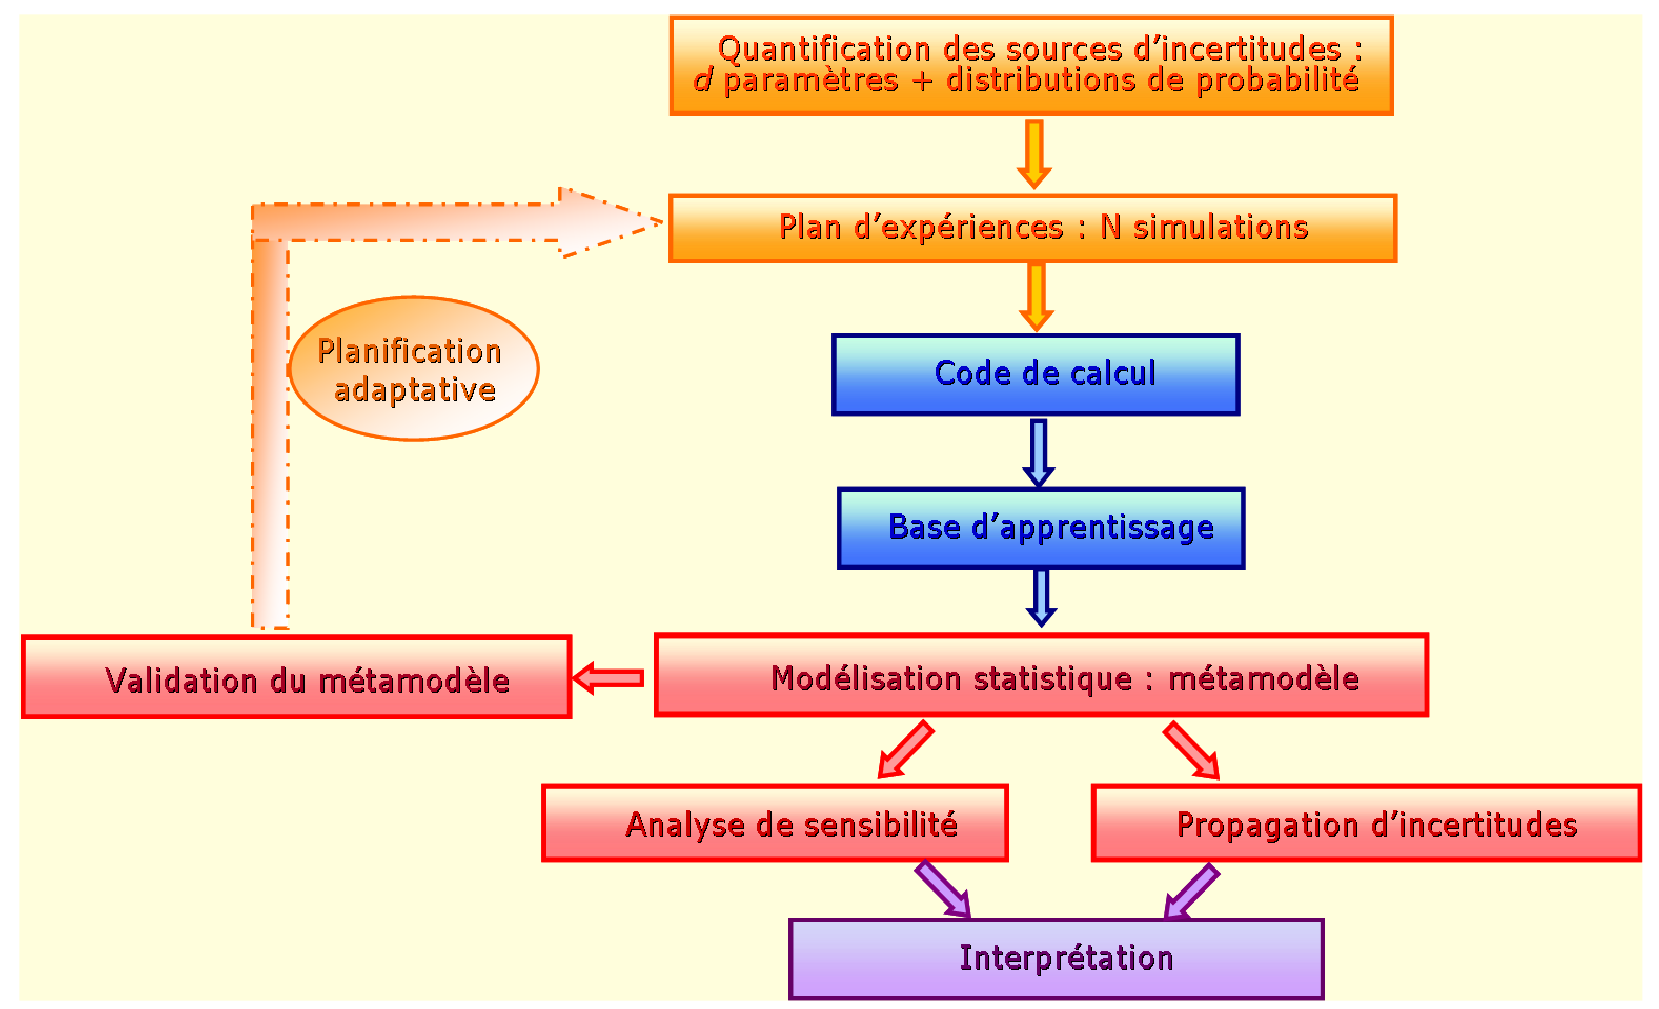
\includegraphics[width=\textwidth]{fig/schemaSeb.png}
\end{frame}

%-----------------------------------------------------------------
\begin{frame}{Pourquoi une stratégie séquentielle ?}
\begin{block}{``Budget'' ($=N$) nécessaire difficile à estimer}
\begin{itemize}
  \item Premier plan raisonnable
  \item Enrichissement jusqu'à satisfaction
\end{itemize}
\end{block}

\begin{alertblock}{Suite d'une première étude}
\begin{itemize}
\item Premier plan $\Rightarrow$ métamodèle grossier $\Rightarrow$ analyse de sensibilité $\Rightarrow$ réduction de dimension
\item Ajout d'expériences pour obtenir un métamodèle final précis
\end{itemize}
\end{alertblock}

\begin{exampleblock}{Planification ciblée $\Leftrightarrow$ utilisation du métamodèle}
\begin{itemize}
\item Propagation d'incertitudes
\item Analyse de sensibilité
\item Optimisation / calibration
\end{itemize}
\end{exampleblock}
\end{frame}
%-----------------------------------------------------------------
\begin{frame}{Approches géométriques vs. métamodèles}

\textbf{Comment ajouter des expériences à un plan existant ?}

\vspace{5mm}

\begin{block}{Approches ``purement'' géométriques}
  \begin{itemize}
  \item Plan factoriels fractionnaires $\Rightarrow$ ajout d'une fraction
  \item Suite à faible discrépance $\Rightarrow$ éléments suivants
  \item Remplissage d'espace (critères \textit{maximin}, \textit{minimax})
 \end{itemize}
$\Rightarrow$ c.f. cours de W. Tinsson, H. Monod et L. Pronzato
\end{block}

\begin{alertblock}{Ici : plans séquentiels \emph{\textit{orientés modèle}}}
 Le métamodèle sert de guide pour choisir les nouvelles observations.
\end{alertblock}
\end{frame}
%-----------------------------------------------------------------
\begin{frame}{Objectifs}
\begin{block}{Cas 1 : métamodèle globalement précis}
Utilisation générique $\Rightarrow$ le métamodèle doit remplacer fidèlement le modèle coûteux
\end{block}

\begin{exampleblock}{Cas 2 : métamodèle = outil d'extraction d'une information}
Intérêt guidé par la valeur des observations
\begin{itemize}
 \item optimisation : recherche de minimum / maximum
 \item analyse de risque : dépassement de seuil
\end{itemize}
Une bonne précision partout n'est pas nécessaire !
\end{exampleblock}
\end{frame}
%-----------------------------------------------------------------